
\documentclass[11pt]{exam} % https://www.ctan.org/pkg/exam?lang=en

\usepackage[lmargin=1.in,rmargin=1.in,tmargin=1.in,bmargin=1in]{geometry}
\usepackage{setspace}
\usepackage[pdftex]{graphicx}
\usepackage{titling}
\usepackage[
	pdfauthor={Brian Weinstein},
	pdftitle={Homework 1},
	bookmarks=true,
	colorlinks=true,
	linkcolor=blue,
	urlcolor=blue,
	citecolor=blue,
	pdftex,
	linktocpage=true
	]{hyperref}
\usepackage[textsize=tiny]{todonotes}
\usepackage{float}
\setlength\parindent{0pt} % or 1em
\usepackage{lipsum}
\usepackage{amsmath}
\usepackage{caption}


\qformat{\textbf{Problem \thequestion: \thequestiontitle}\quad \hfill}


\pagestyle{headandfoot}
\runningheadrule
\firstpageheader{}{}{}
\runningheader{\theauthor}{\thetitle}{\thedate}
\firstpagefooter{}{\thepage}{}
\runningfooter{}{\thepage}{}


\usepackage{xcolor}
\usepackage{adjustbox}
\usepackage{verbatim}
\definecolor{shadecolor}{rgb}{.9, .9, .9}

\newenvironment{code}%
   {\par\noindent\adjustbox{margin=1ex,bgcolor=shadecolor,margin=0ex \medskipamount}\bgroup\minipage\linewidth\verbatim}%
   {\endverbatim\endminipage\egroup}

\newenvironment{codeSmall}%
   {\par\noindent\adjustbox{margin=1ex,bgcolor=shadecolor,margin=0ex \medskipamount}\bgroup\minipage\linewidth\verbatim\footnotesize}%
   {\endverbatim\endminipage\egroup}

\newcommand{\ramsey}{\href{http://www.statisticalsleuth.com/}{Ramsey }}



\begin{document}


\title{STAT W4201 001, Homework 7}
\author{Brian Weinstein (bmw2148)}
\date{Mar 28, 2016}
\maketitle

Code is attached here and also posted at \href{https://github.com/BrianWeinstein/advanced-data-analysis}{https://github.com/BrianWeinstein/advanced-data-analysis}. Where relevant, code snippets and output are are included in-line.

\begin{questions}


\titledquestion{\ramsey 10.21}
\setlength{\parindent}{1em}

Let

$$
\mathbf{Y} = 
  \begin{bmatrix}
    Y_1 \\
    Y_2 \\
    \vdots \\
    Y_n
  \end{bmatrix}
, \quad
\mathbf{X}=
  \begin{bmatrix}
    1 & X_{11} & X_{12} & \cdots & X_{1p} \\
    1 & X_{21} & X_{22} & \cdots & X_{2p} \\
    \vdots & \vdots & \vdots &  & \vdots \\
    1 & X_{n1} & X_{n2} & \cdots & X_{np} \\
  \end{bmatrix}
, \quad \text{and \ }
\mathbf{b} = 
  \begin{bmatrix}
    \beta_0 \\
    \beta_1 \\
    \vdots \\
    \beta_p
  \end{bmatrix} .
$$

By deconstructing $(\mathbf{X}^T \mathbf{X}) \mathbf{b} = \mathbf{X}^T \mathbf{Y}$ we find the set of normal equations:
\begin{gather*}
(\mathbf{X}^T \mathbf{X}) \mathbf{b} = \mathbf{X}^T \mathbf{Y} \\ 
\Rightarrow \left(
  \begin{bmatrix}
  	1 & 1 & \cdots & 1 \\
  	X_{11} & X_{21} & \cdots & X_{n1} \\
  	X_{12} & X_{22} & \cdots & X_{n2} \\
    \vdots & \vdots &  & \vdots \\
  	X_{1p} & X_{2p} & \cdots & X_{np} \\
  \end{bmatrix}
  \begin{bmatrix}
    1 & X_{11} & X_{12} & \cdots & X_{1p} \\
    1 & X_{21} & X_{22} & \cdots & X_{2p} \\
    \vdots & \vdots & \vdots &  & \vdots \\
    1 & X_{n1} & X_{n2} & \cdots & X_{np} \\
  \end{bmatrix}
\right)
\begin{bmatrix}
    \beta_0 \\
    \beta_1 \\
    \vdots \\
    \beta_p
  \end{bmatrix}
=
  \begin{bmatrix}
  	1 & 1 & \cdots & 1 \\
  	X_{11} & X_{21} & \cdots & X_{n1} \\
  	X_{12} & X_{22} & \cdots & X_{n2} \\
    \vdots & \vdots &  & \vdots \\
  	X_{1p} & X_{2p} & \cdots & X_{np} \\
  \end{bmatrix}
  \begin{bmatrix}
    Y_1 \\
    Y_2 \\
    \vdots \\
    Y_n
  \end{bmatrix}
\\
\Rightarrow \begin{bmatrix}
  	n & \sum X_{i1} & \sum X_{i2} & \cdots & \sum X_{ip} \\
  	\sum X_{i1} & \sum X_{i1}^2 & \sum X_{i1} X_{i2 } & \cdots & \sum X_{i1} X_{ip} \\
  	\sum X_{i2} & \sum X_{i2} X_{i1} & \sum X_{i2}^2 & \cdots & \sum X_{i2} X_{ip} \\
  	\vdots & \vdots & \vdots &  & \vdots \\
  	\sum X_{ip} & \sum X_{ip} X_{i1} & \sum X_{ip} X_{i2} & \cdots & \sum X_{ip}^2 \\
  \end{bmatrix}
  \begin{bmatrix}
    \beta_0 \\
    \beta_1 \\
    \vdots \\
    \beta_p
  \end{bmatrix}
=
  \begin{bmatrix}
    \sum Y_{i} \\
    \sum X_{i1} Y_i \\
    \sum X_{i2} Y_i \\
    \vdots \\
    \sum X_{ip} Y_i \\
  \end{bmatrix}
\\
\Rightarrow \begin{bmatrix}
  	\beta_0 n + \beta_1 \sum X_{i1} + \beta_2 \sum X_{i2} + \cdots + \beta_p \sum X_{ip} \\
  	\beta_0 \sum X_{i1} + \beta_1 \sum X_{i1}^2 + \beta_2 \sum X_{i1} X_{i2 } + \cdots + \beta_p \sum X_{i1} X_{ip} \\
  	\beta_0 \sum X_{i2} + \beta_1 \sum X_{i2} X_{i1} + \beta_2 \sum X_{i2}^2 + \cdots + \beta_p \sum X_{i2} X_{ip} \\
  	\vdots \\
  	\beta_0 \sum X_{ip} + \beta_1 \sum X_{ip} X_{i1} + \beta_2 \sum X_{ip} X_{i2} + \cdots + \beta_p \sum X_{ip}^2 \\
  \end{bmatrix}
=
  \begin{bmatrix}
    \sum Y_{i} \\
    \sum X_{i1} Y_i \\
    \sum X_{i2} Y_i \\
    \vdots \\
    \sum X_{ip} Y_i \\
  \end{bmatrix} ,
\end{gather*}
where each $\sum$ indicates summation over all cases ($i = 1, 2, \ldots, n$).

As long as $\mathbf{X}^T \mathbf{X}$ is invertible, the least squares solution is $\mathbf{b} = (\mathbf{X}^T \mathbf{X})^{-1} \mathbf{X}^T \mathbf{Y}$. By the invertible matrix theorem, $\mathbf{X}^T \mathbf{X}$ is invertible whenever the columns of $\mathbf{X}$ are linearly independent.

\titledquestion{\ramsey 10.22}
\setlength{\parindent}{1em}

\textit{Continuing Exercise 21, statistical theory says that the means of the estimates in the vector $\mathbf{A} \mathbf{Y}$, where $\mathbf{A}$ is a matrix, are the elements of the vector $\mathbf{A} \mu \{\mathbf{Y}\}$; and the matrix of covariances of these estimates is $\mathbf{A} \text{Cov}(\mathbf{Y})\mathbf{A}^T$.}

\begin{parts}

\part \textit{Use the theory and the model $\mu \{\mathbf{Y}\} = \mathbf{X} \beta$; $\text{Cov}(\mathbf{Y}) = \sigma^2 \mathbf{I}$ (where $\mathbf{I}$ is an $n \times n$ identity matrix) to show that the mean in the sampling distributions of the least squares estimate $\mathbf{b}$ is $\beta$.}

\begin{align*}
\text{E}\left[ \mathbf{b} \right] &= \text{E}\left[ (\mathbf{X}^T \mathbf{X})^{-1} \mathbf{X}^T (\mathbf{Y}) \right] \\
&= \text{E}\left[ (\mathbf{X}^T \mathbf{X})^{-1} \mathbf{X}^T (\mathbf{X} \beta) \right] \\
&= \text{E}\left[ (\mathbf{X}^T \mathbf{X})^{-1} (\mathbf{X}^T \mathbf{X}) \beta \right] \\
&= \text{E}\left[ \mathbf{I} \beta \right] \\
&= \text{E}\left[ \beta \right] \\
&= \beta
\end{align*}


\part \textit{Then show that the matrix of covariances is $\text{Cov}\{\mathbf{b}\} = \sigma^2 (\mathbf{X}^T \mathbf{X})^{-1}$.}








\end{parts}

\titledquestion{\ramsey 10.26}
\setlength{\parindent}{1em}

\textit{Does the effect of UVB exposure on the distribution of percentage inhibition differ at the surface and in the deep? How much difference is there? Analyze the data, and write a summary of statistical findings and a section of details documenting those findings.}

A sample of the dataset is shown below, and a coded scatterplot of the \texttt{Inhibit} vs \texttt{UVB} is shown in Figure \ref{fig:3_eda}.

\begin{codeSmall}
   Inhibit  UVB Surface
1      0.0 0.00       0
2      1.0 0.00       0
3      6.0 0.01       0
4      7.0 0.01       1
...
14    21.0 0.04       1
15    25.0 0.02       0
16    39.0 0.03       0
17    59.0 0.03       0
\end{codeSmall}

\begin{figure}[!h]
	\centering
	\captionsetup{width=0.8\textwidth}
	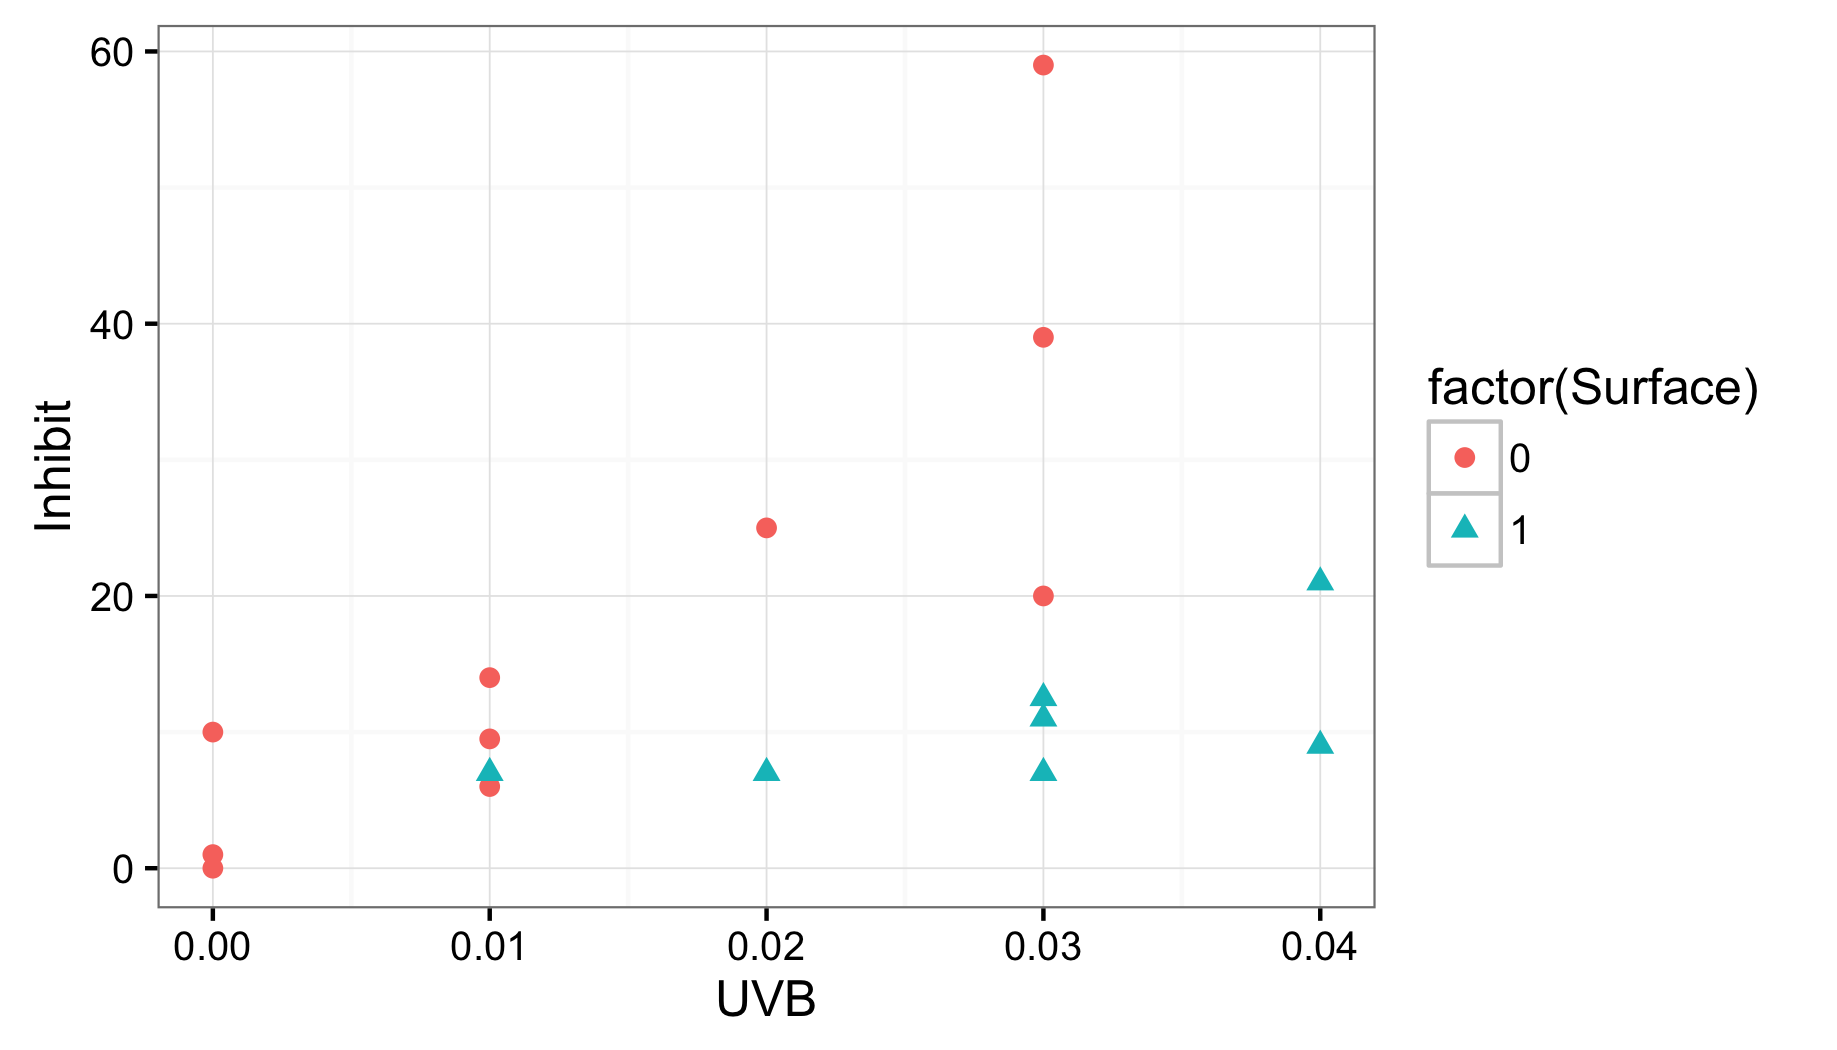
\includegraphics[width=4.25in]{3_eda.png}
	\caption{Coded scatterplot of \texttt{Inhibit} vs \texttt{UVB}. \texttt{Surface} = 1 indicates a measurement close to the surface, and \texttt{Surface} = 0 in deep water.}
	\label{fig:3_eda}
\end{figure}

First, we fit a linear model on the full dataset, including an interaction term between \texttt{UVB} and \texttt{Surface}.

\begin{codeSmall}
> lmFull <- lm(Inhibit ~ Surface*UVB, data=ozoneData)
> summary(lmFull)$coefficients
               Estimate Std. Error    t value     Pr(>|t|)
(Intercept)    1.180556   4.292122  0.2750517 0.7875994449
Surface        1.277778  11.065902  0.1154698 0.9098372976
UVB         1226.388889 232.772995  5.2686047 0.0001518894
Surface:UVB -939.930556 409.839150 -2.2934133 0.0391340538
\end{codeSmall}$

In this model, the p-value on the intercept term indicates that the data provides no evidence to suggest that the intercept is non-zero. Based on the dataset, we also know the intercept should be nearly 0 for both the surface-level and deep water measurements. We fit a second model, forcing the intercept term to 0.

\begin{codeSmall}
> lmZeroInt <- lm(Inhibit ~ 0 + Surface*UVB, data=ozoneData)
> summary(lmZeroInt)$coefficients
               Estimate Std. Error    t value      Pr(>|t|)
Surface        2.458333   9.857139  0.2493962 0.80667620946
UVB         1275.000000 146.400333  8.7089966 0.00000050281
Surface:UVB -988.541667 357.358785 -2.7662442 0.01515365491
\end{codeSmall}$

Although the model with 0-intercept has a slightly higher RMSE, the difference is negligible (8.537, vs 8.833 in the full model), and the significance of the coefficients is unchanged.

Based on the full model, the data provides moderate evidence that the effect of UVB exposure on the distribution of percentage inhibition differs at the surface and in the deep (two sided p-value of $0.03913$, from a test that the \texttt{Surface:UVB} coefficient estimate is 0; estimated value $-939.9$, 95\% CI from -1825 to -54.53). In deep water, for each 0.01 unit increase in UVB exposure, the percent inhibition increases by 12.26 percentage points. Near the surface, however, for each 0.01 unit increase in UVB exposure, the percent inhibition increases by only 2.861 percentage points.

The regression equations for this ``separate lines'' model are shown below
\begin{itemize}
\item Near the surface ($\texttt{Surface} = 1$): $\texttt{Inhibit} = 3.084 + 286.1 \times \texttt{UVB}$,
\item and in deep water ($\texttt{Surface} = 0$): $\texttt{Inhibit} = 1.806 + 1226 \times \texttt{UVB}$.
\end{itemize}

\titledquestion{\ramsey 11.8}
\setlength{\parindent}{1em}

\begin{parts}
\setlength{\parindent}{1em}

\part \textit{Why does a case with large leverage have the potential to be influential? Why is it not necessarily influential?}

An observation with large leverage $h_i$ has a residual with low variability
$$\text{SD}(\text{Residual}_i) = \sigma \sqrt{1-h_i}.$$ A high-leverage observation's explanatory variable values are abnormally high or low, as compared to the other observations in the dataset. As such, the high-leverage observation determines the value of the regression in the surrounding region.

This, however, does not mean that all high-leverage observations are influential. If the observation happens to fall close to the regression surface that is fit only to the other observations (i.e., excluding the high-leverage observation), then the high-leverage observation has little impact on the overall regression surface.

\part \textit{Draw a hypothetical scatterplot of Y versus a single X, where one observation has a high leverage but is not influential.}

A scatterplot with a high-leverage, low-influence observation is shown in Figure \ref{fig:4b}.

\begin{figure}[!h]
	\centering
	\captionsetup{width=0.8\textwidth}
	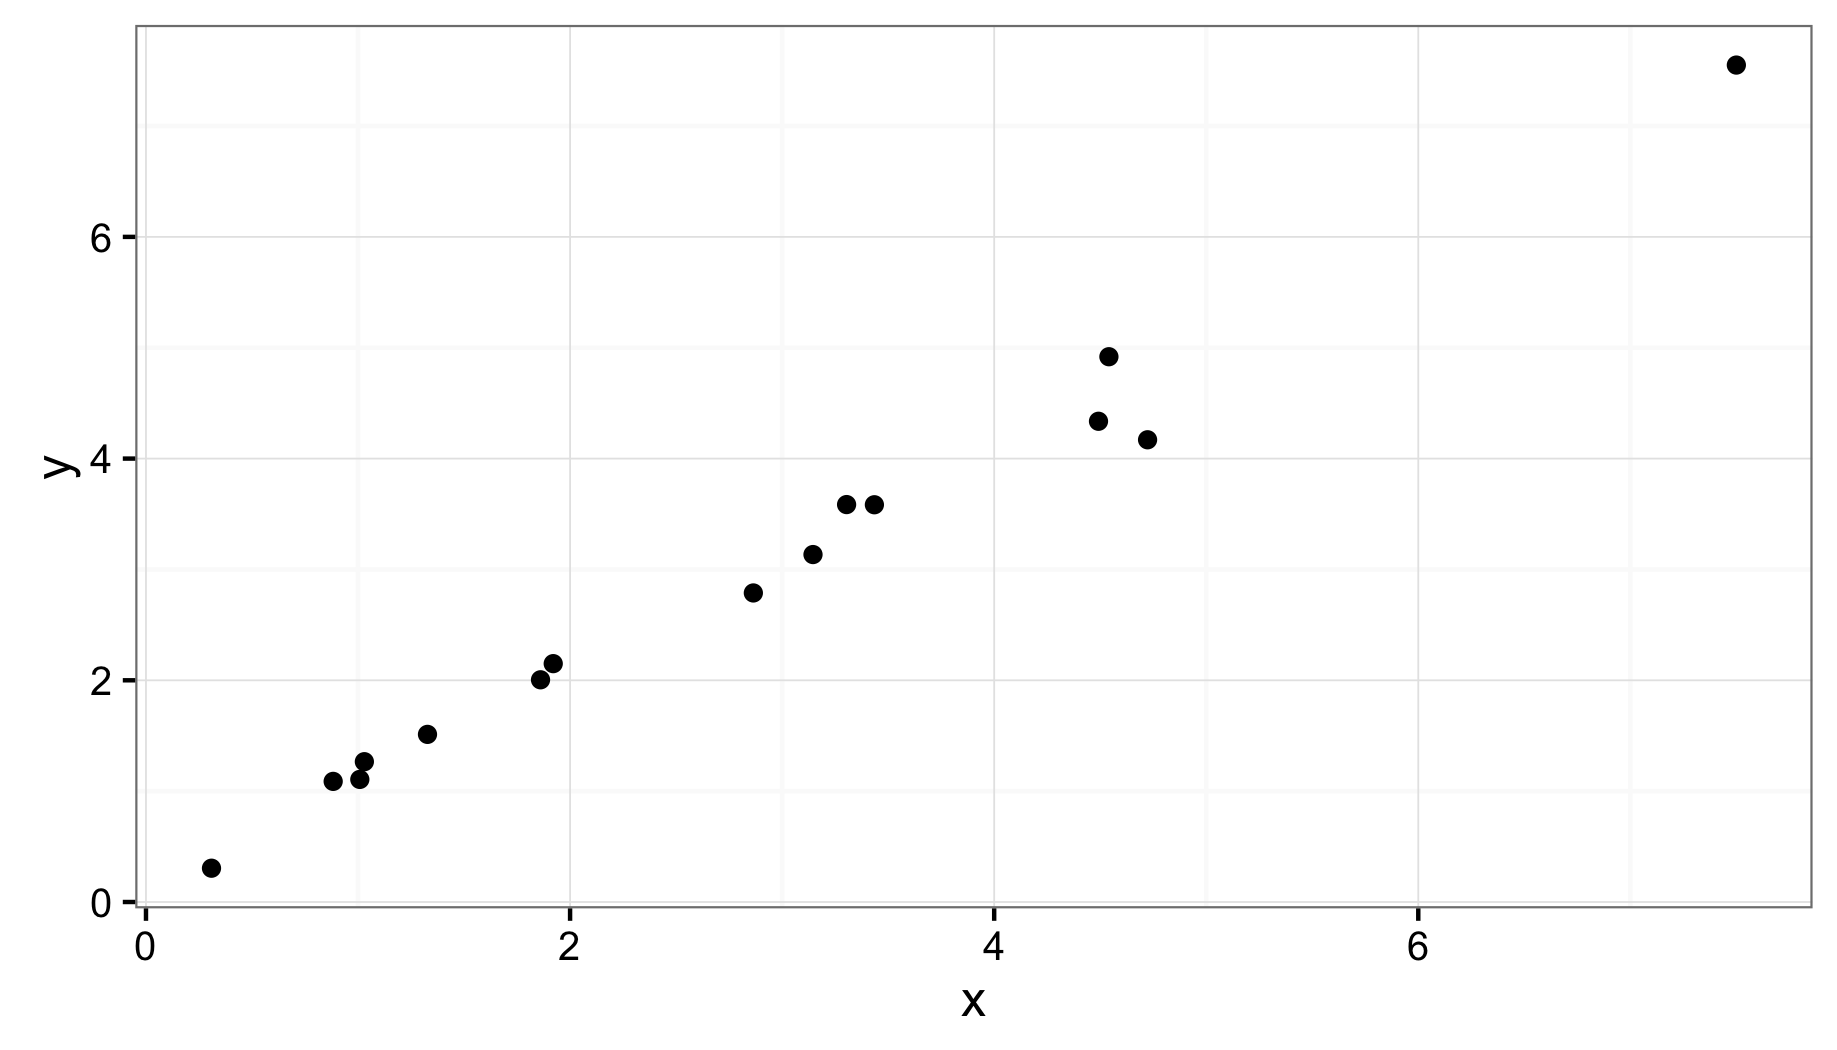
\includegraphics[width=4in]{4b.png}
	\caption{A scatterplot with a high-leverage, low-influence observation.}
	\label{fig:4b}
\end{figure}

\part \textit{Draw a hypothetical scatterplot of Y versus a single X, where one observation has a high leverage and is influential.}

A scatterplot with a high-leverage, high-influence observation is shown in Figure \ref{fig:4c}.

\begin{figure}[!h]
	\centering
	\captionsetup{width=0.8\textwidth}
	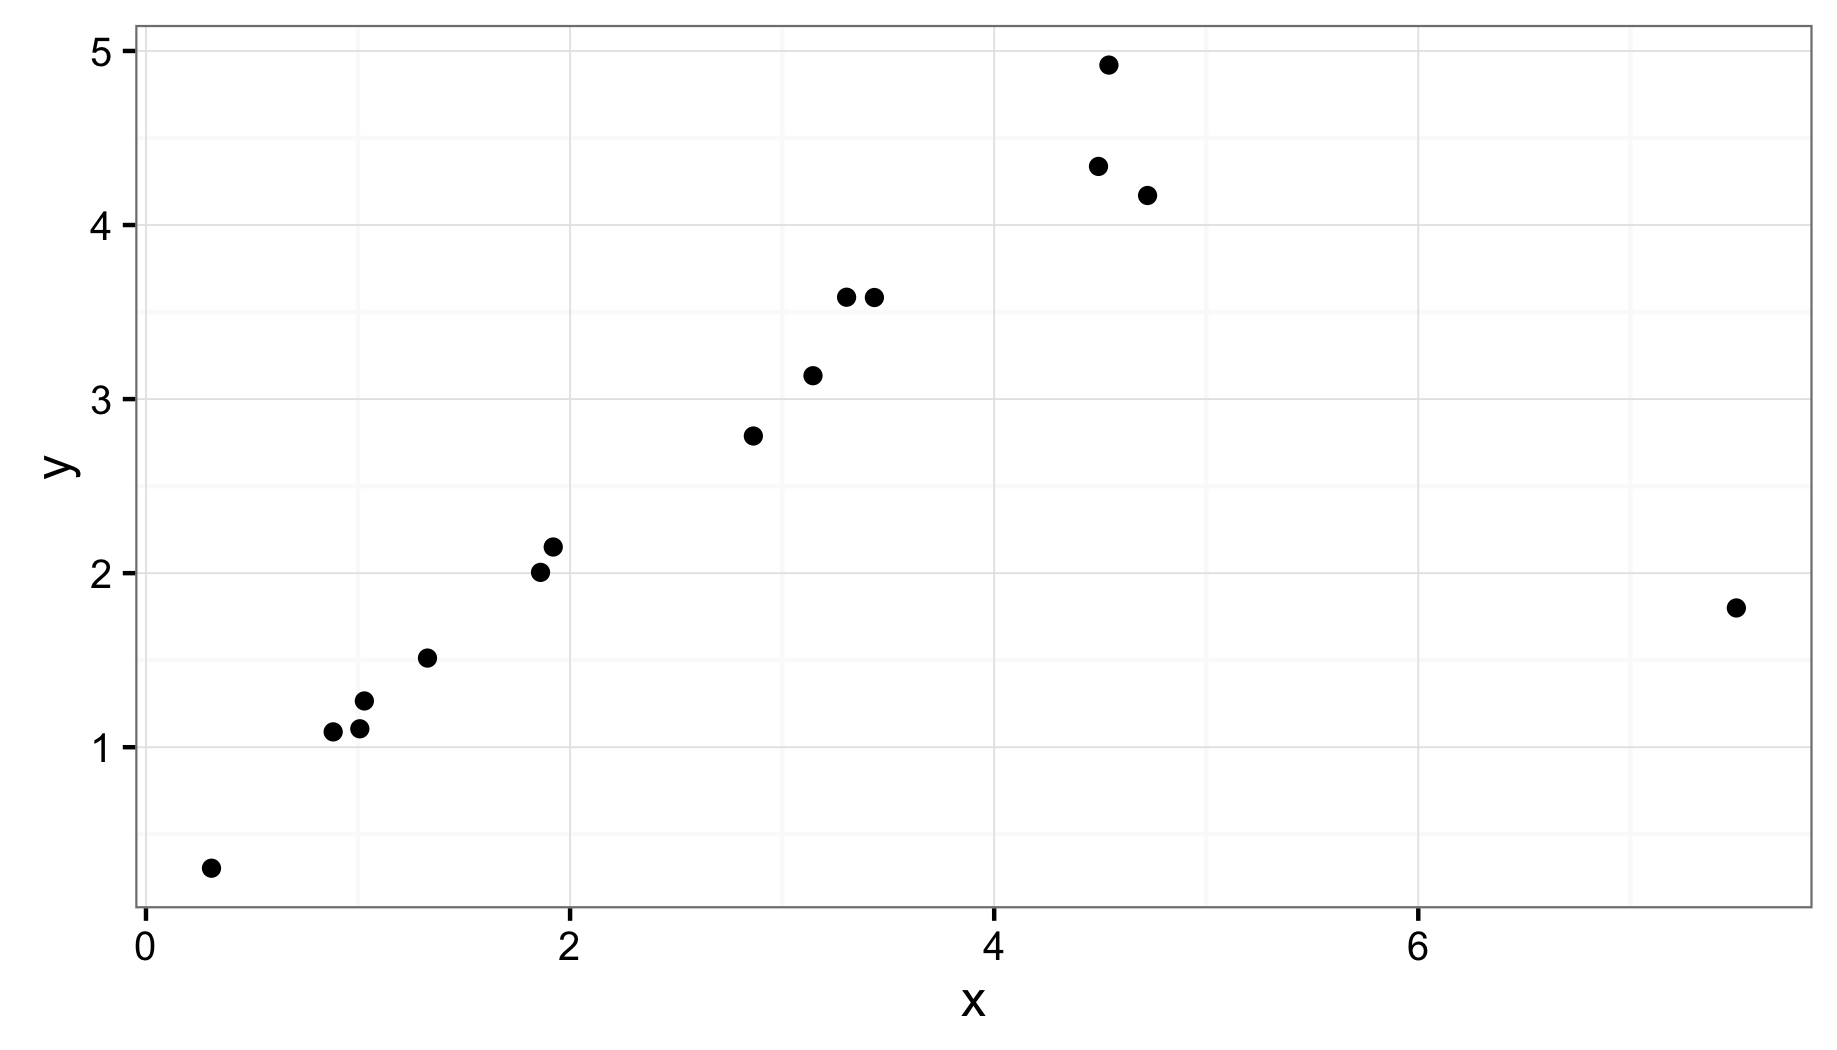
\includegraphics[width=4in]{4c.png}
	\caption{A scatterplot with a high-leverage, high-influence observation.}
	\label{fig:4c}
\end{figure}

\end{parts}

\titledquestion{\ramsey 11.16}
\setlength{\parindent}{1em}


\textit{Calculate the leverage, the studentized residual, and Cook’s Distance for the 32nd case. Use the model with gastric activity, a sex indicator variable, and the interaction of these two.}

The regression of \texttt{Metabol} on \texttt{Gastric}, \texttt{Sex}, and their interaction is shown below, and a coded scatterplot is shown in Figure \ref{fig:5}.

\begin{codeSmall}
> lmFpm <- lm(formula = Metabol ~ Gastric*Sex, data = fpmData)
> summary(lmFpm)$coefficients
                  Estimate Std. Error    t value   Pr(>|t|)
(Intercept)     -0.1972691  0.8022017 -0.2459096 0.80754593
Gastric          0.8369478  0.4838925  1.7296153 0.09471027
SexMale         -0.9884969  1.0723910 -0.9217691 0.36452374
Gastric:SexMale  1.5069236  0.5591376  2.6950856 0.01176490
\end{codeSmall}$

\begin{figure}[!h]
	\centering
	\captionsetup{width=0.8\textwidth}
	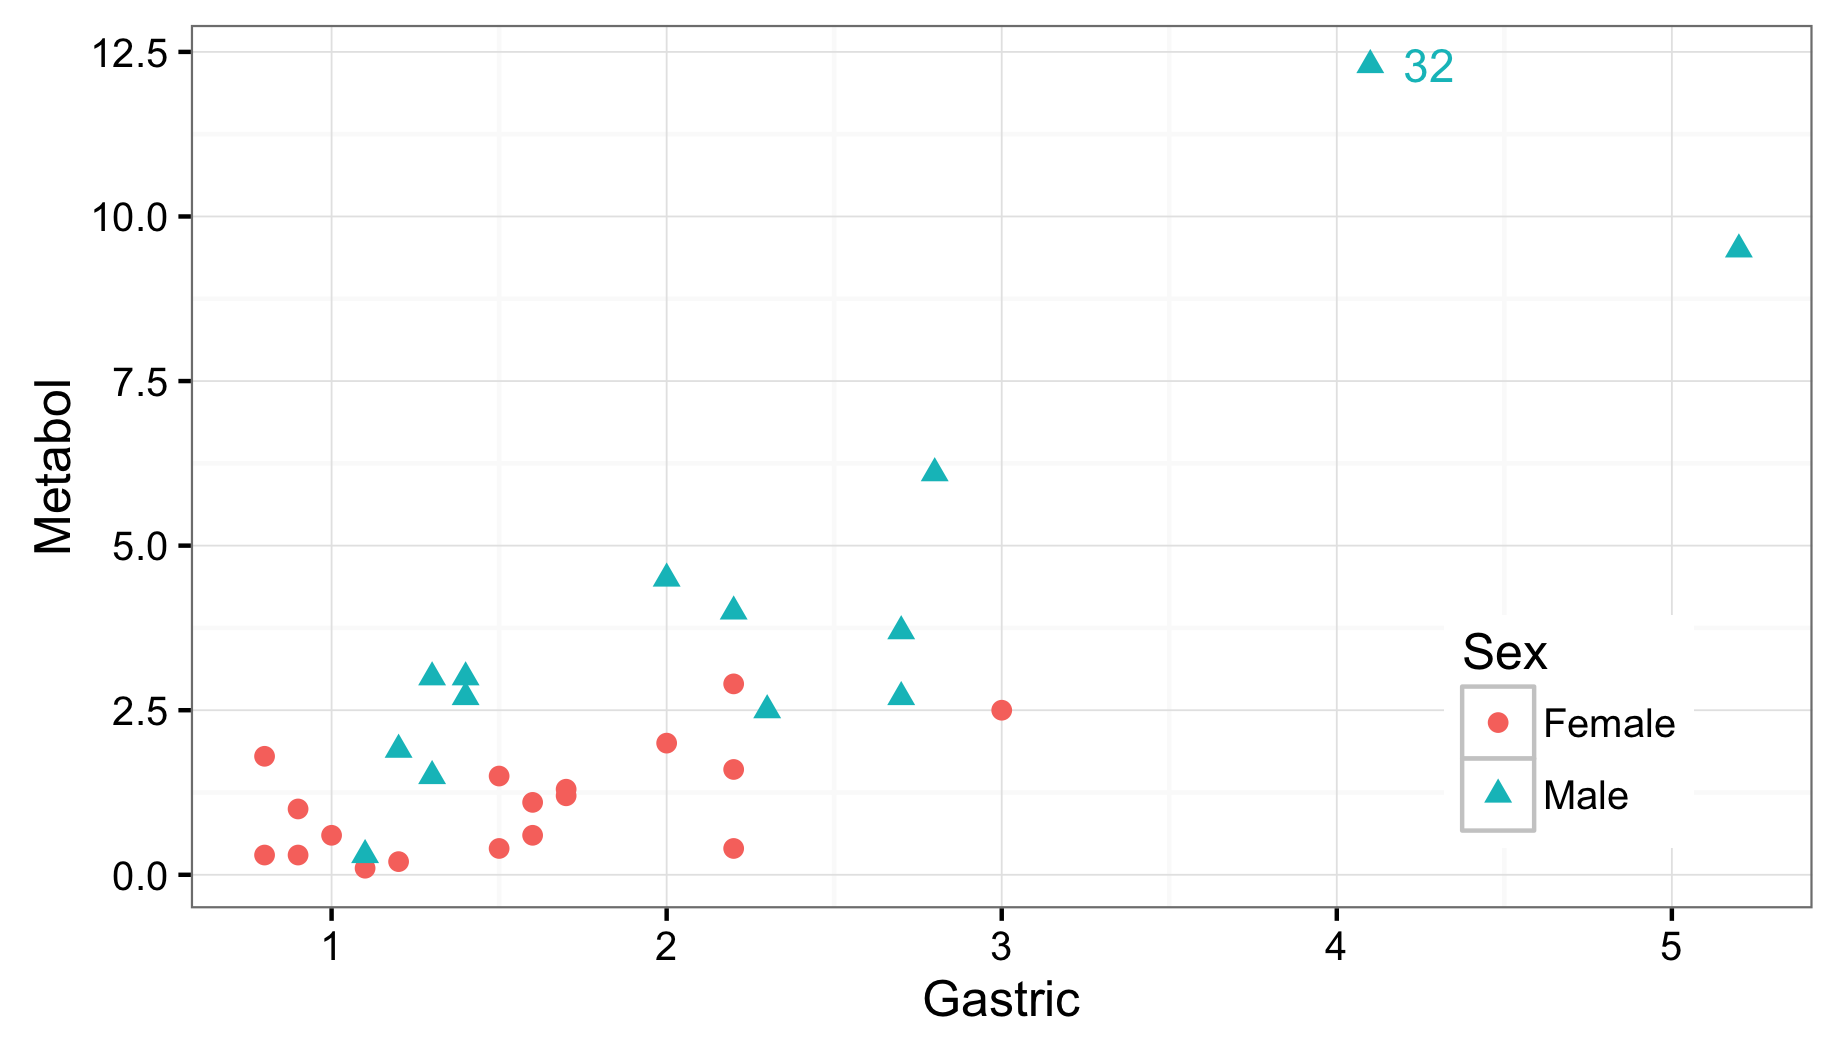
\includegraphics[width=4.25in]{5.png}
	\caption{Coded scatterplot of \texttt{Metabol} vs \texttt{Gastric}.}
	\label{fig:5}
\end{figure}

The leverage, studentized residual, and Cook's Distance for case 32 are shown below.
\begin{codeSmall}
> # calculate leverage for case 32
> hatvalues(lmFpm)[32]
       32 
0.2528749 
> # calculate the studentized residual for case 32
> studres(lmFpm)[32]
      32 
5.120516 
> # calculate Cook's Distance for case 32
> cooks.distance(lmFpm)[32]
      32 
1.167255 
\end{codeSmall}


\titledquestion{\ramsey 11.20}
\setlength{\parindent}{1em}


\begin{parts}
\setlength{\parindent}{1em}


\part \textit{Examine the effects on the p-value for significance of regression and on R-squared of deleting (i) the case with the smallest value of X, and (ii) the two cases with the smallest values of X.}

The relevant portions of the linear model summary outputs are shown below.

\begin{itemize}


\item Model 1 (full dataset):
\begin{codeSmall}
Residual standard error: 0.9959 on 16 degrees of freedom
Multiple R-squared:  0.8427,	Adjusted R-squared:  0.8329 
F-statistic: 85.73 on 1 and 16 DF,  p-value: 0.00000007929
\end{codeSmall}

With the full dataset, the p-value for the overall significance of regression (i.e., the p-value based on the F-statistic, which is the same as the p-value associated with the slope estimate for simple linear regression), is $7.929 \times 10^{-8}$, and the R-squared is $0.8427$.


\item Model 2 (dataset excluding the case with the smallest value of X):
\begin{codeSmall}
Residual standard error: 0.9807 on 15 degrees of freedom
Multiple R-squared:  0.6718,	Adjusted R-squared:  0.6499 
F-statistic:  30.7 on 1 and 15 DF,  p-value: 0.00005653
\end{codeSmall}

By removing the case with the smallest value of X, the p-value of $5.653 \times 10^{-5}$ still indicates that there's overwhelming evidence of an association between Calcite and Carbonate, but it is three orders of magnitude smaller than in Model 1 . The R-squared has also decreased to $0.6718$.


\item Model 3 (dataset excluding the two cases with the smallest values of X):
\begin{codeSmall}
Residual standard error: 0.8875 on 14 degrees of freedom
Multiple R-squared:  0.3398,	Adjusted R-squared:  0.2926 
F-statistic: 7.205 on 1 and 14 DF,  p-value: 0.0178
\end{codeSmall}

By removing the two cases with the smallest values of X, the p-value of $0.0178$ is still significant, but is considerably smaller than in Models 1 and 2. The R-squared has also decreased even further to $0.2926$.

\end{itemize}


\part \textit{Why does R-squared change so much?}

The two cases with the smallest values of X also have the two smallest values of Y, and significantly increase the overall variation in the Y variable. By removing the smallest value of X in Model 2 (and then also the second-smallest value of X in Model 3), the total variation in Y decreases significantly, but the residual sum of squares doesn't change very much.

The total sum of squares and residual sum of squares for the 3 models are shown below.
\begin{codeSmall}
> # compare total and residual sum of squares for lmFull
> sum(anova(lmFull)$"Sum Sq")
[1] 100.9
> (anova(lmFull)$"Sum Sq")[2]
[1] 15.86942
> 
> # compare total and residual sum of squares for lmExcl1
> sum(anova(lmExcl1)$"Sum Sq")
[1] 43.95882
> (anova(lmExcl1)$"Sum Sq")[2]
[1] 14.42715
> 
> # compare total and residual sum of squares for lmExcl2
> sum(anova(lmExcl2)$"Sum Sq")
[1] 16.70438
> (anova(lmExcl2)$"Sum Sq")[2]
[1] 11.02839
\end{codeSmall}

The R-squared statistic is defined as $(1 - \frac{\text{Residual Sum of Squares}}{\text{Total Sum of Squares}})$, so with the total sum of squares decreasing so dramatically from Model 1 to Models 2 and 3, but the residual sum of squares staying more or less the same, the R-squared statistic decreases dramatically when the two smallest X values are removed.


\part \textit{Compute the case influence statistics, and discuss interesting cases.}

Plots of the case influence statistics are shown in Figure \ref{fig:6c}, and a scatterplot of Calcite vs Carbonate is shown in Figure \ref{fig:6c_scatter}.

\begin{figure}[!h]
	\centering
	\captionsetup{width=0.8\textwidth}
	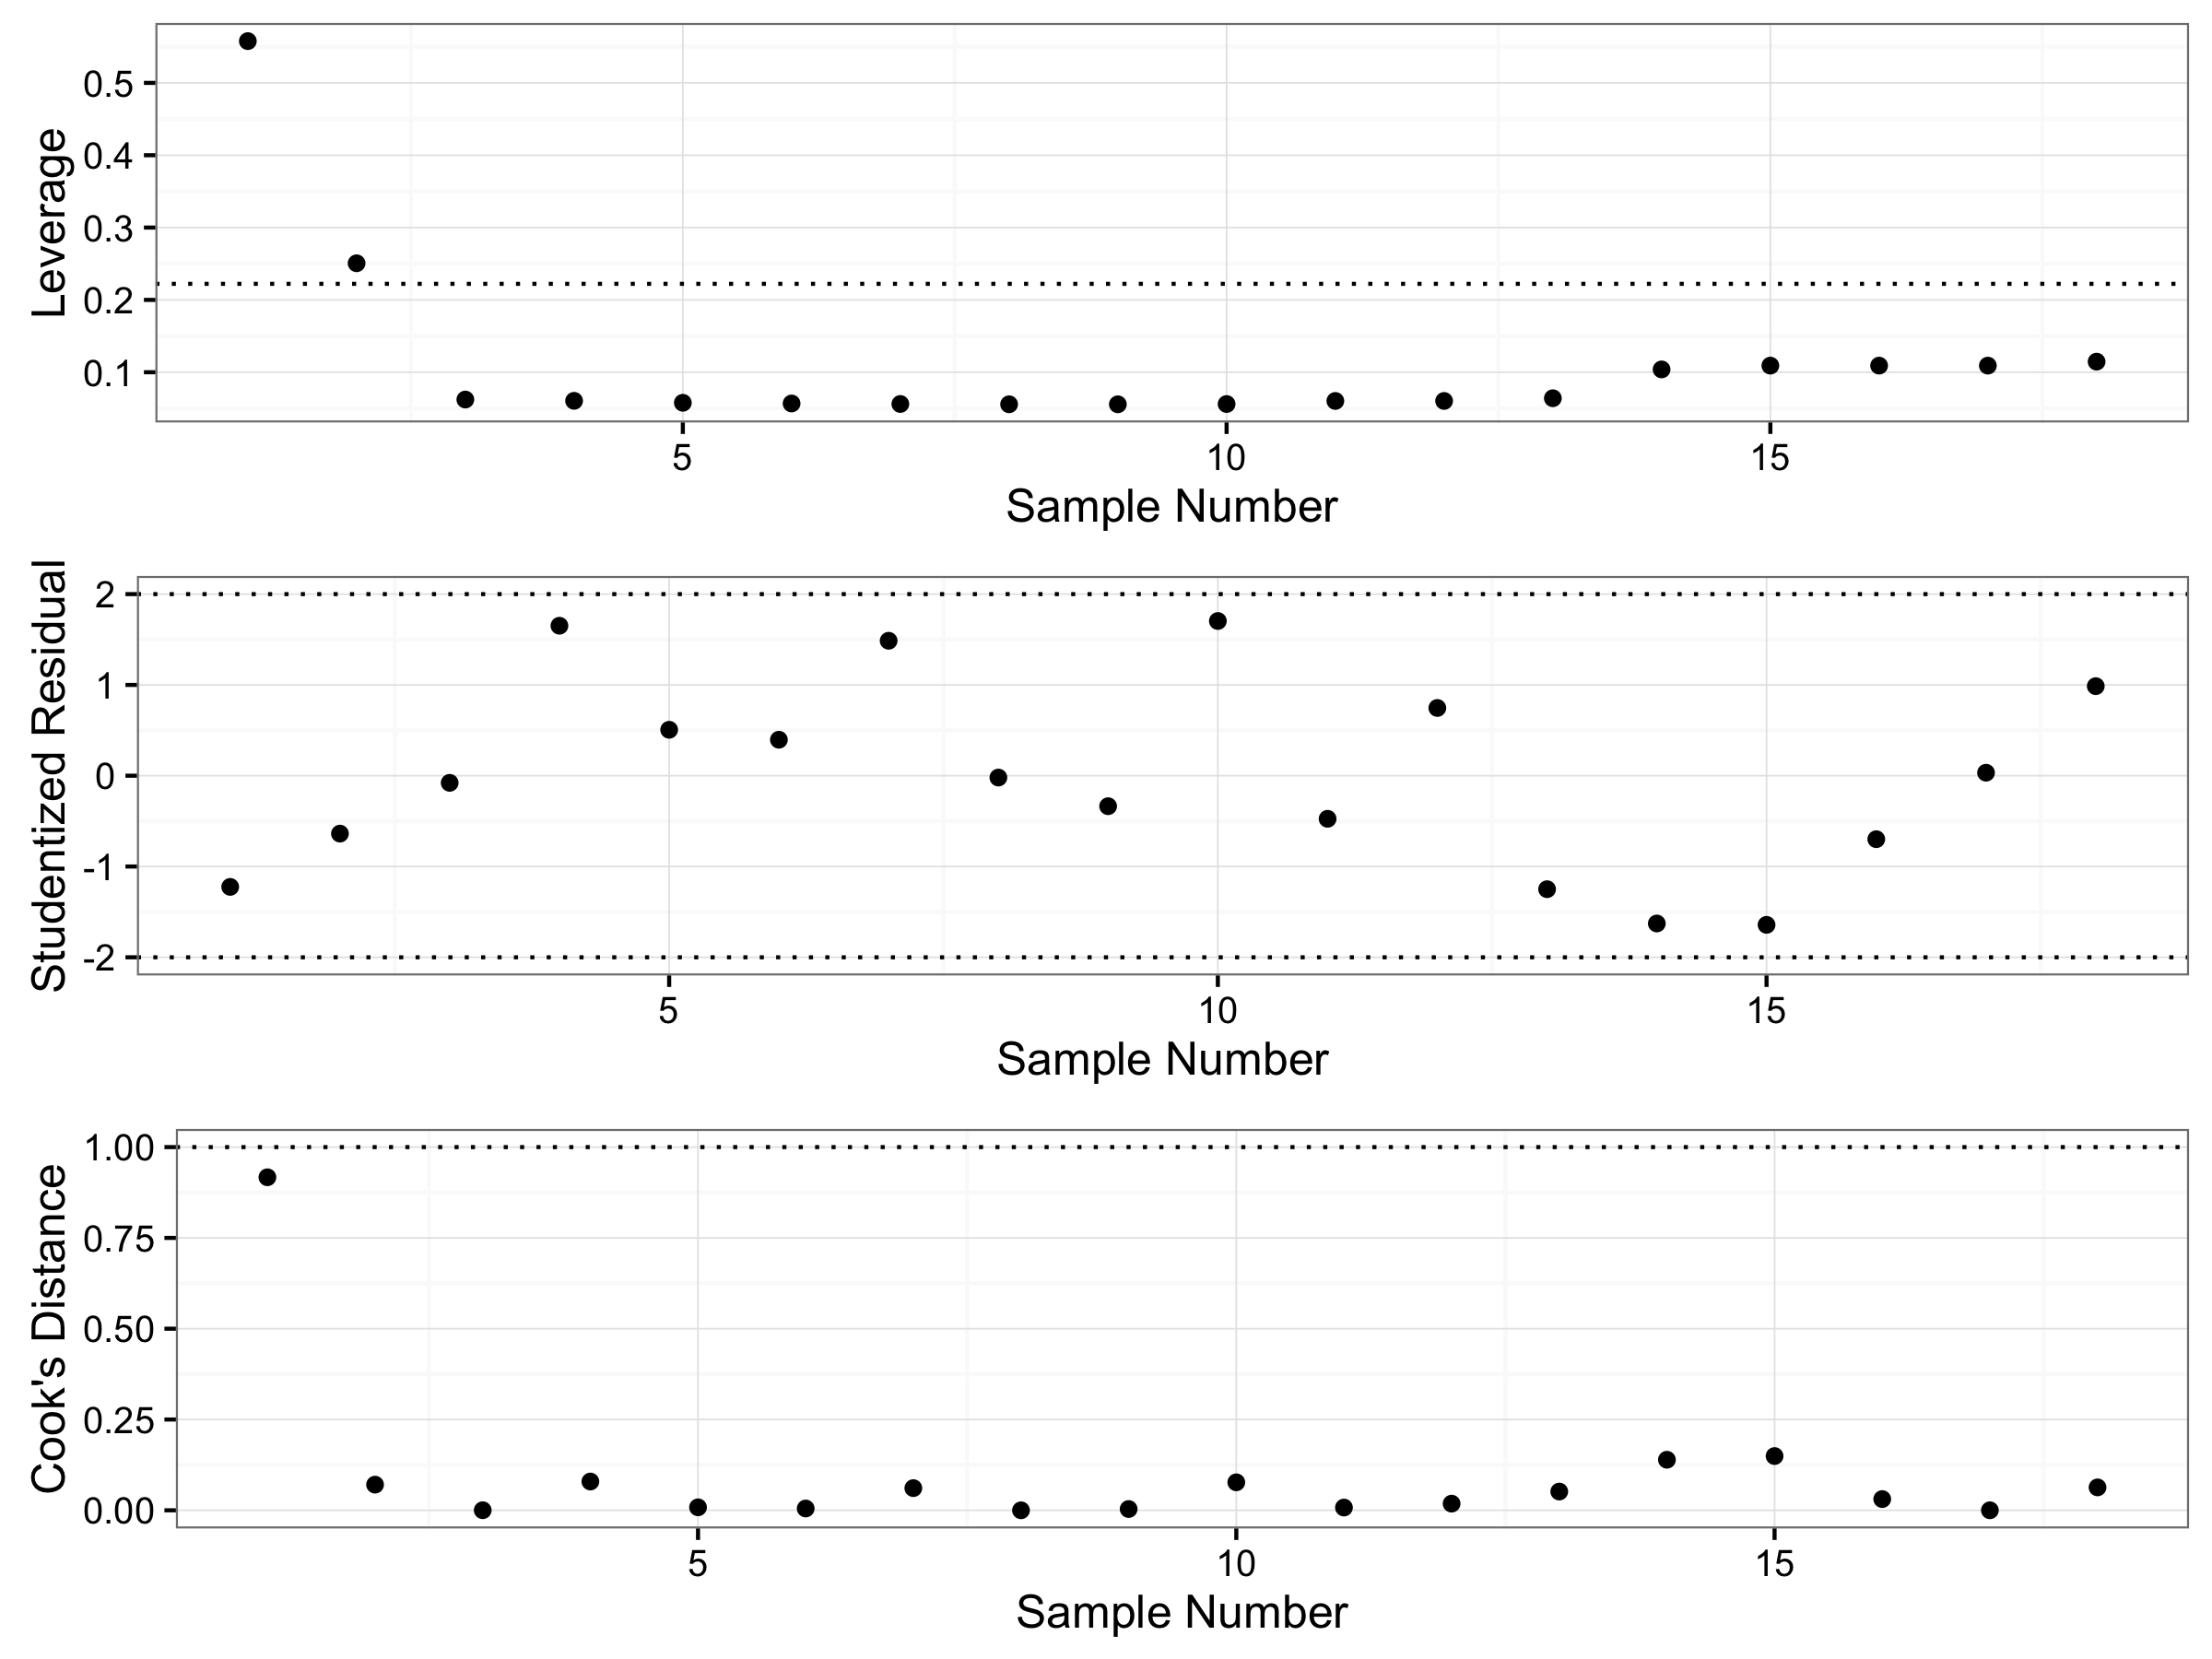
\includegraphics[width=5.5in]{6c.png}
	\caption{Plots of the leverage statistics, studentized residuals, and Cook's Distances for each observation in the regression of Calcite on Carbonate, using the full dataset.}
	\label{fig:6c}
\end{figure}

\begin{figure}[!h]
	\centering
	\captionsetup{width=0.8\textwidth}
	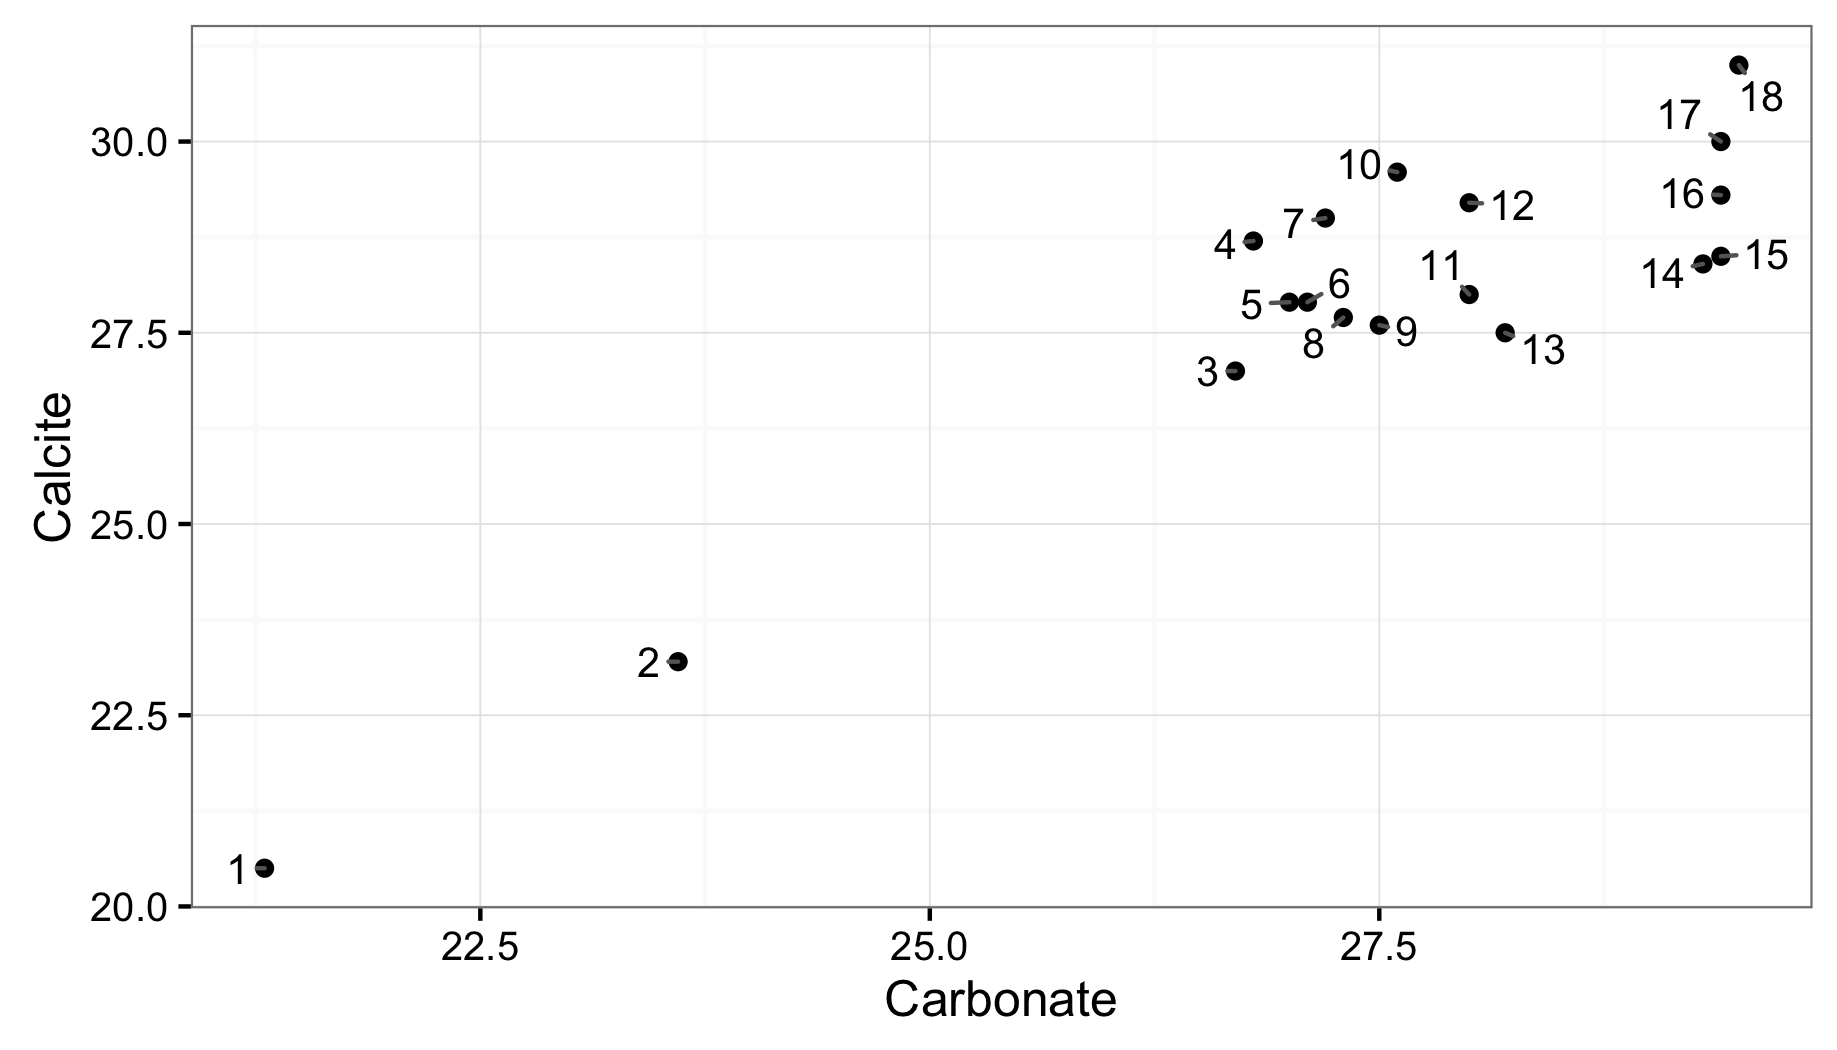
\includegraphics[width=4.25in]{6c_scatter.png}
	\caption{Scatterplot of Calcite vs Carbonate with points labeled by the Sample Number, corresponding to the Sample Number in Figure \ref{fig:6c}.}
	\label{fig:6c_scatter}
\end{figure}

Cases 1 and 2 have leverages that are greater than $(\text{2 times the average leverage}) = (2 \times p/n) = (2 \times 2/18) = 0.222$, so they warrant further attention. Neither Case 1 nor Case 2 have abnormal studentized residuals. Based on its large leverage, Case 1 has a large Cook's Distance, however, and is thus an influential observation.

Cases 4, 7, 10, 14, and 15 have studentized residuals moderately far from zero, but not enough to cause concern, especially in light of their small Cook's Distances.

\part \textit{Recompute the case statistics when the case with the smallest X is deleted.}

Plots of the case influence statistics are shown in Figure \ref{fig:6d}.

\begin{figure}[!h]
	\centering
	\captionsetup{width=0.8\textwidth}
	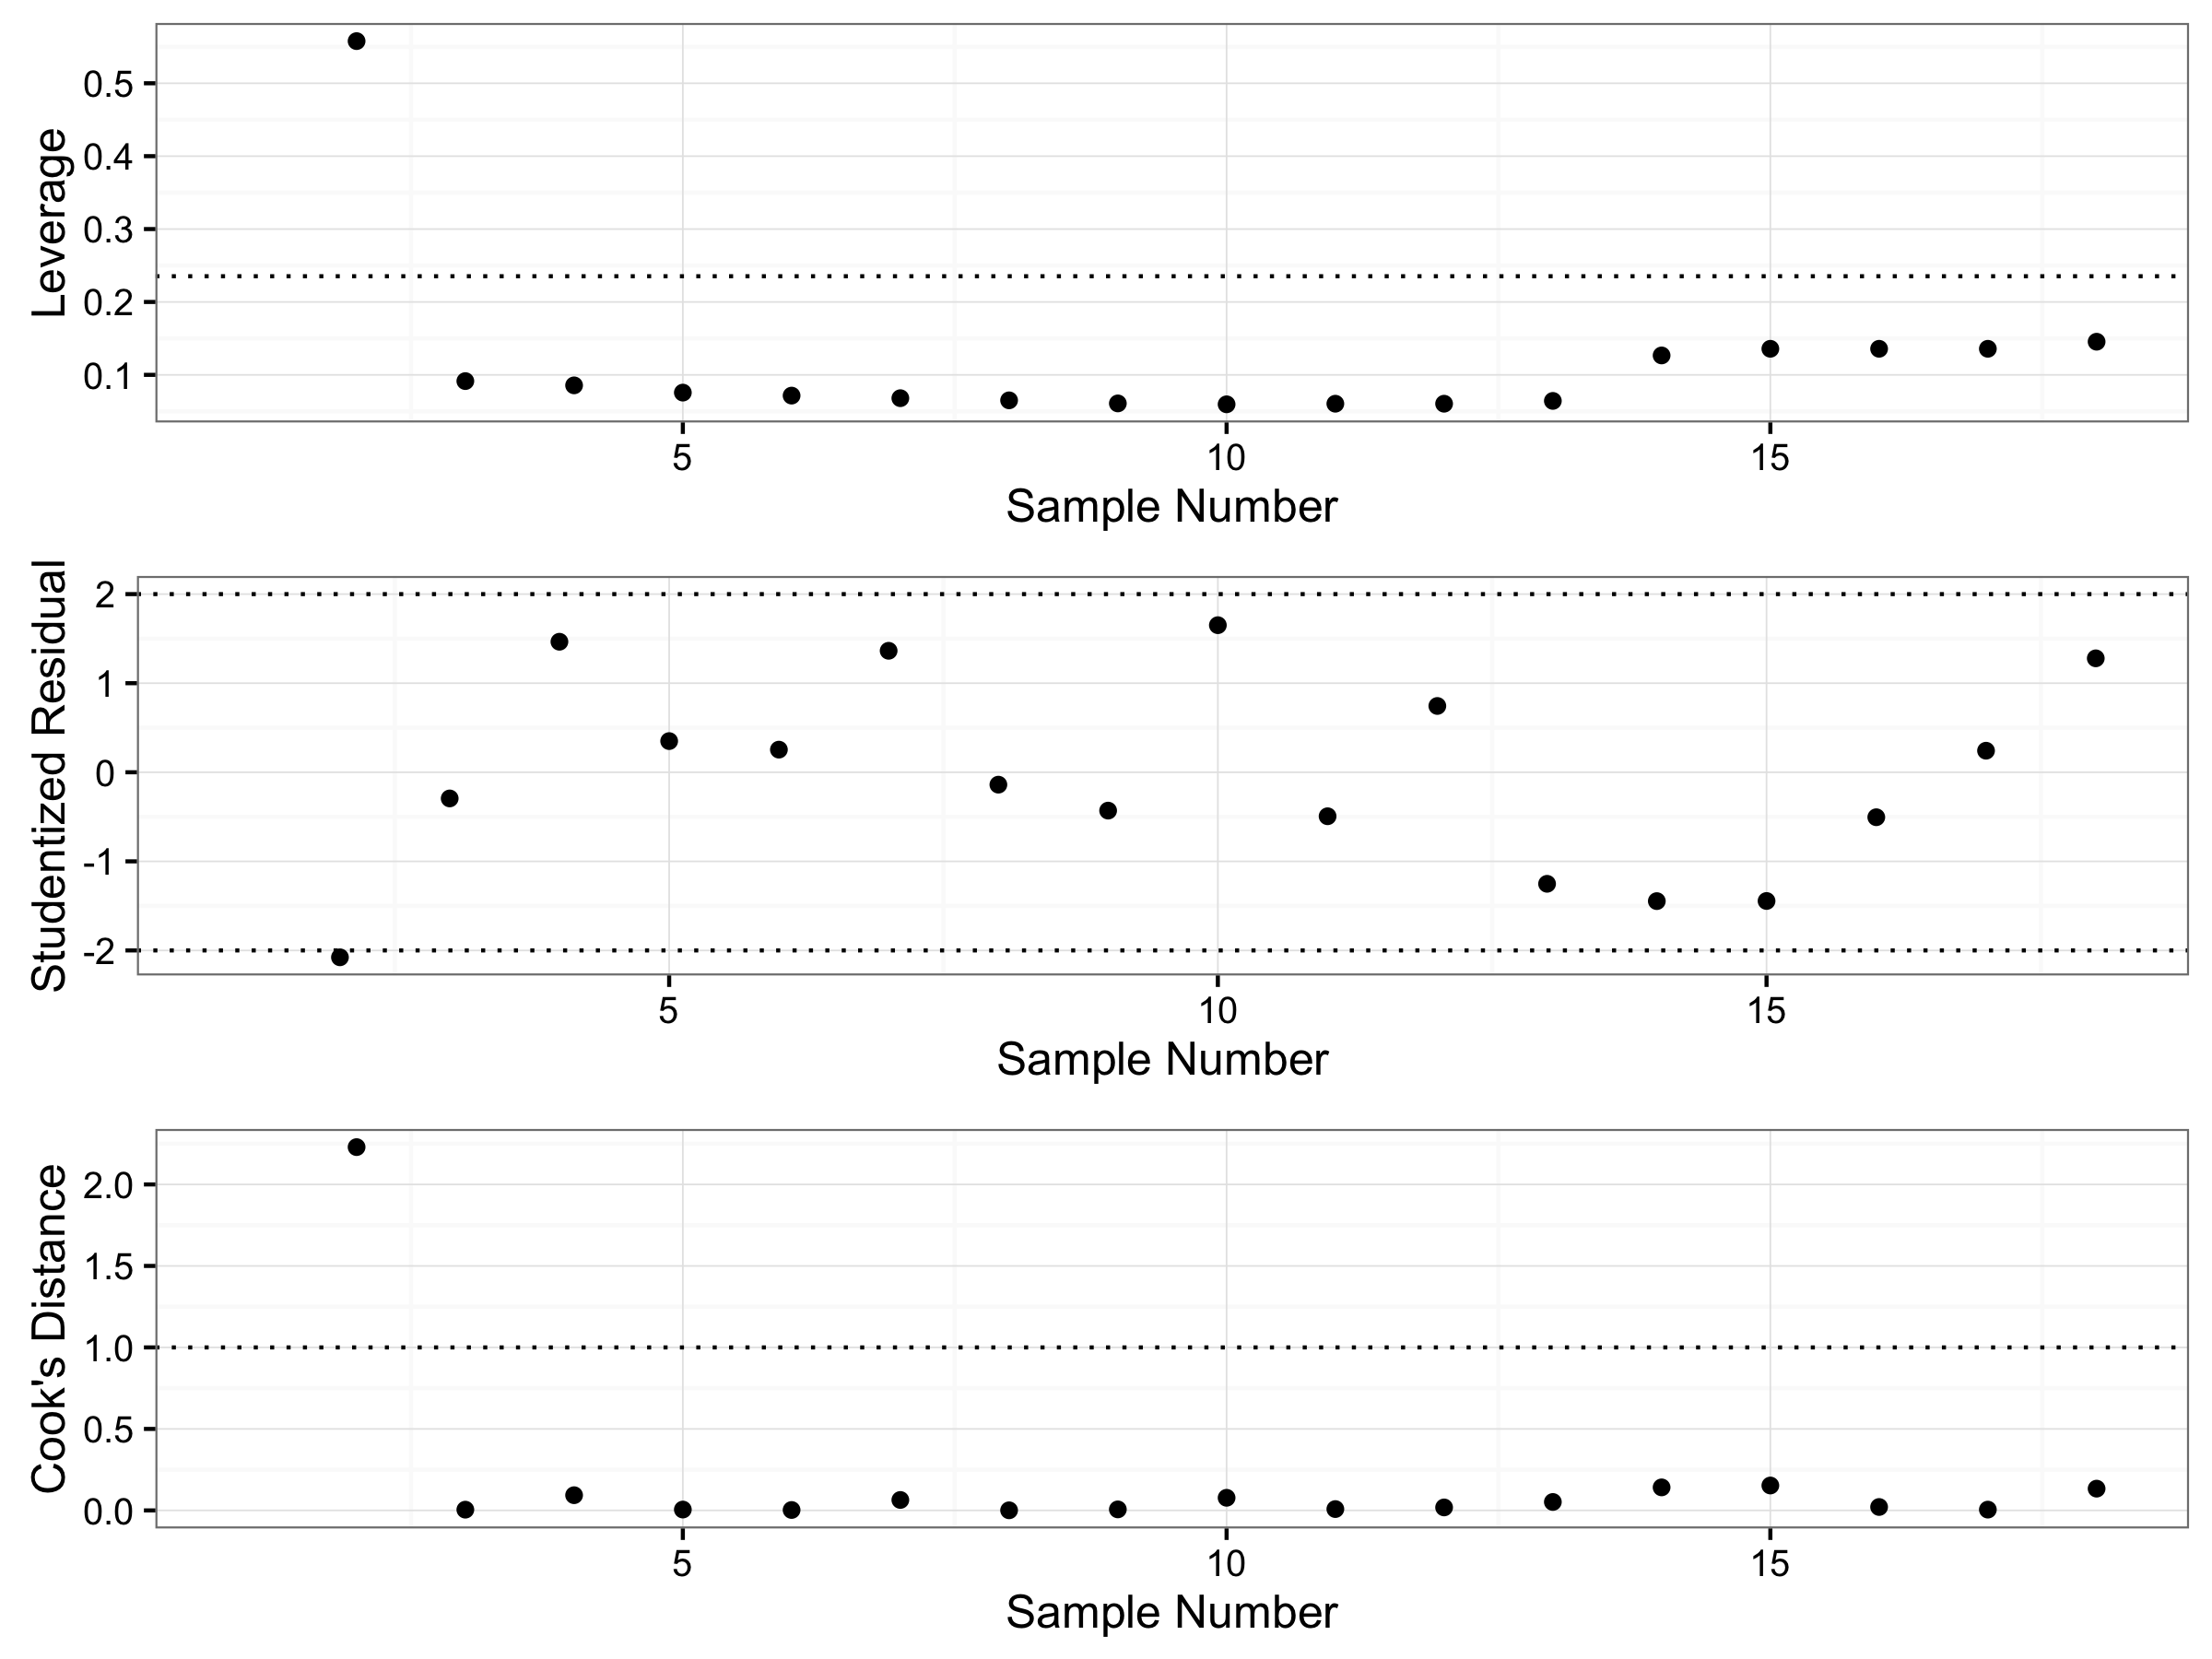
\includegraphics[width=5.5in]{6d.png}
	\caption{Plots of the leverage statistics, studentized residuals, and Cook's Distances for each observation in the regression of Calcite on Carbonate, using the dataset with the smallest X excluded.}
	\label{fig:6d}
\end{figure}

\part \textit{Comment on the differences in the two sets of case statistics. Why may pairs of influential observations not be found with the usual case influence statistics?}

After removing the observation with the smallest X (Case 1) from the dataset, the leverage of Case 2 significantly increased and is now much greater than $(\text{2 times the average leverage}) = (2 \times p/n) = (2 \times 2/17) = 0.235$. Case 2 now also has a studentized residual far enough from zero to cause concern. A vale of $2.23$ for Cook's Distance indicates that Case 2 has high influence on the regression coefficients.

In general, pairs of influential observations may not be found with the usual case influence statistics. This is because the presence of the most extreme case can make other observations --- ones which aren't as extreme as the \textit{most} extreme case, but may seem extreme after this case is removed --- seem more or less average.

With all observations included, the mean $X$ value, $\overline{X}$, is shifted toward the most extreme case (Case 1, in this example). As such, $\overline{X}$ is also shifted towards the slightly less extreme Case 2, and the overall leverage of Case 2 is decreased.

$$h_i = \frac{1}{n} + \frac{1}{n-1} \left[ \frac{X_i - \overline{X}}{s_X}  \right]^2$$

Once the most extreme case is removed, however, $\overline{X}$ moves closer towards the other observations, but further away from Case 2, now making Case 2 have an alarmingly high leverage.

\part \textit{What might one conclude about the influence of the two unusual observations in this data set?}

As noted in parts (c) and (e), both Case 1 and Case 2 have high influence over the regression coefficients.



\end{parts}


\end{questions}

\listoftodos

\end{document}